\documentclass[11pt]{article}
\usepackage[margin=1in]{geometry}
\usepackage[T1]{fontenc}
\usepackage[utf8]{inputenc}
\usepackage{lmodern}
\usepackage{microtype}
\usepackage{amsmath,amssymb,mathtools}
\usepackage{booktabs,tabularx,array,longtable}
\usepackage{enumitem}
\usepackage{graphicx}
\usepackage{tikz}
\usetikzlibrary{arrows.meta,positioning,shapes.geometric,fit,calc}
\usepackage{pgfplots}
\pgfplotsset{compat=1.18}
\usepgfplotslibrary{groupplots}
\usepackage[hidelinks]{hyperref}
\usepackage[nameinlink,noabbrev]{cleveref}
\usepackage{caption}
\setlength{\parindent}{1.2em}
\setlength{\parskip}{0.35em}
\renewcommand{\arraystretch}{1.15}
\newcommand{\FSS}{\mathcal{S}}
\newcommand{\CSR}{\operatorname{CSR}}
\newcommand{\Risk}{\mathcal{R}}
\newcommand{\Status}{\mathcal{S}_R}
\newcommand{\Defeat}{\mathcal{D}}

\title{Claim-Status Routing and Shape-Scaled Sparse-Prior Risk Analysis:\\
Second-Order Risk Management Under Threat-Coupled Gatekeeping}
\author{Author omitted for blind review}
\date{June 2026}

\begin{document}
\maketitle

\begin{abstract}
Severe-if-true risks can become decision-relevant before stable frequencies, mature analogues, calibrated models, or ordinary institutional routines exist. At that boundary, risk management can fail before it misestimates probability: it can lose the candidate object before ordinary assessment begins. This Perspective proposes \emph{claim-status routing}, a second-order protocol that preserves, types, routes, and updates sparse-prior candidates without treating admission as validation, forecast, or intervention authorization. It represents a risk as a risk-relevant shape on a fitness-conceptual topology projection, and represents that shape as a typed graph of boundaries and admissible transitions. The graph supplies a piecewise constraint algebra: existing risk-management methods can be composed across the regions in which they are valid without presuming a unifying model of the entire domain. Predicted shapes may be stored in typed risk-shape libraries before empirical registration, provided their expected signatures, bridge obligations, blocked uses, and stopping conditions remain explicit. This permits reuse of constraints, monitoring plans, and routing operations, not transfer of empirical truth, probability, severity, or decision authority. The protocol distinguishes local objections from parent defeat, unsafe evidence routes from safe decision objects, and artifact retention from regenerative propagation of a complete safety case. The companion supplement gives the formal reconstruction, including completion-invariant constraints, compatibility-preserving library reuse, and a bounded Lean routing kernel. The framework is pre-validation infrastructure: it aims to deliver a better-preserved object to ordinary empirical, institutional, and decision processes rather than replace them.
\end{abstract}

\section{Introduction: the second-order risk problem}
\label{sec:introduction}

Risk analysis has developed substantial methods for evaluating uncertainty once a risk object has entered an assessment frame: formal risk characterization, expert elicitation, model validation, exploratory modeling, robust decision making, dynamic adaptive policy pathways, sensitivity analysis, and risk governance \cite{kaplan1981,cooke1991,bankes1993,lempert2003,benhaim2006,haasnoot2013,marchau2019,renn2008}. This Perspective addresses a prior boundary. A candidate may be novel, adaptive, severe if true, and sparse in frequencies or mature analogues. It may be difficult to formulate as a stable scenario precisely because its adequate formulation is among the things at issue. Before ordinary assessment can begin, the candidate must survive a more basic operation: preservation as a correctly typed object.

The distinction is between two failures:
\begin{align}
\text{first-order failure} & = \text{misassessment of an admitted risk object}, \\
\text{second-order failure} & = \text{failure to preserve or correctly type the object before assessment}.
\end{align}

A second-order failure can be locally procedurally defensible. A carrier may be weak; a diagram may be schematic; a venue may be unsuitable; evidence may be immature; a decision use may be unjustified; a method may be difficult to operationalize; or a claim may be emotionally and institutionally high-valence. Each can justify a real downstream consequence. The structural failure occurs when one of these local consequences is silently substituted for \emph{projection defeat}: a defeat of the parent risk object, its map, a load-bearing interface, or its claimed global relation.

\begin{figure}[htbp]
\centering
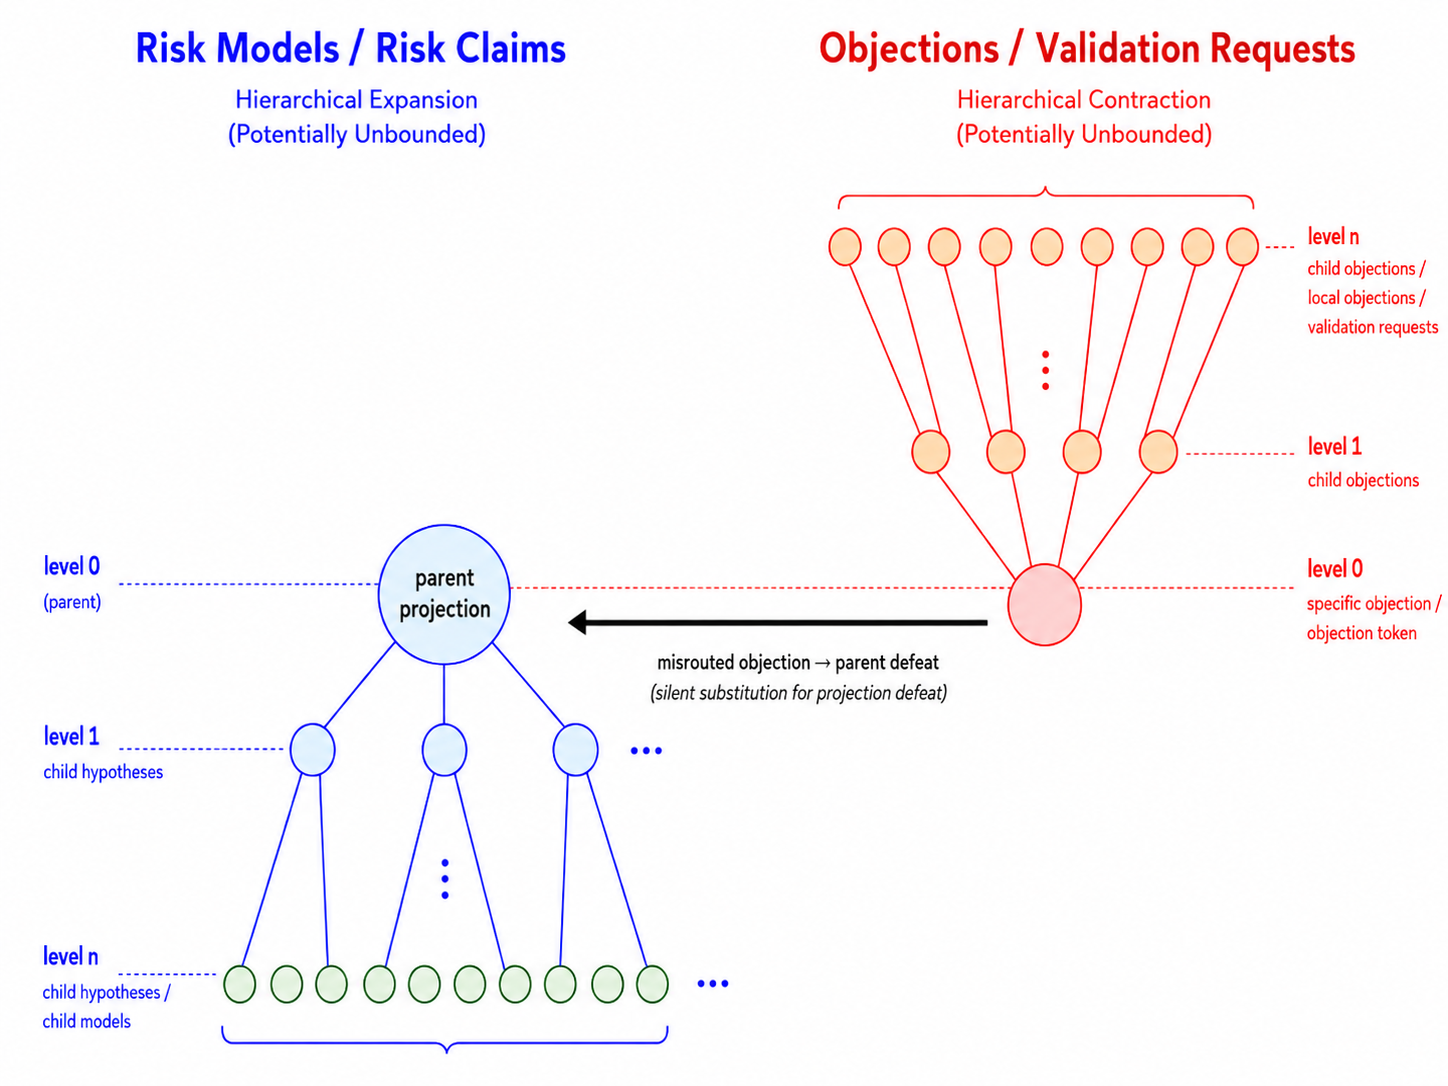
\includegraphics[width=0.98\textwidth]{risk_v87_hierarchy.png}
\caption{\textbf{Potentially unbounded expansion and contraction around a parent projection.} A continuous formal model of risk can generate an unbounded family of globally coherent child hypotheses, just as the continuous equation $r^2=x^2+y^2+z^2$ defines unboundedly many points on a sphere in real-valued Euclidean space. Requests to empirically validate, refine, localize, or challenge those child hypotheses can likewise generate an unbounded family of objections. The left hierarchy represents expansion from a parent projection into child hypotheses or models; the right hierarchy represents contraction from potentially unbounded local objections or validation requests toward a particular objection token. The shared level-$0$ line makes visible the failure mode: a local objection can be silently substituted for defeat of the parent projection. Claim-status routing contains this infinite instability by preserving the parent, typing each objection, routing it only to its permitted coordinate, and requiring a finite, targeted, contradiction-establishing witness before parent defeat is entered.}
\label{fig:hierarchy-expansion-contraction}
\end{figure}

The paper's contribution is deliberately bounded. It does not validate an AI-pause thesis, establish a Great Filter forecast, prove a current governance collapse, recommend a policy, or replace domain-specific risk assessment. It specifies a pre-validation routing discipline intended to ensure that a severe-if-true sparse-prior candidate can reach the appropriate downstream assessment process without being either promoted to belief or erased by status substitution.

\begin{figure}[htbp]
\centering
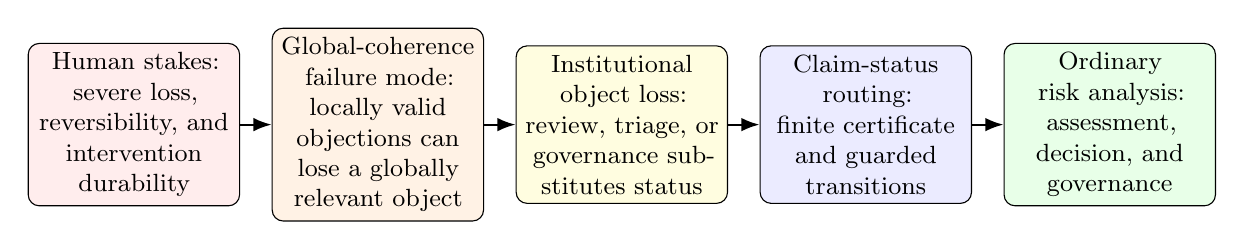
\begin{tikzpicture}[node distance=0.75cm and 0.4cm, every node/.style={font=\small}, box/.style={draw, rounded corners, align=center, minimum height=0.85cm, text width=2.45cm}, arr/.style={-Latex,thick}]
\node[box,fill=red!7] (stakes) {Human stakes:\\severe loss, reversibility, and intervention durability};
\node[box,fill=orange!10,right=of stakes] (shape) {Global-coherence failure mode:\\locally valid objections can lose a globally relevant object};
\node[box,fill=yellow!12,right=of shape] (loss) {Institutional object loss:\\review, triage, or governance substitutes status};
\node[box,fill=blue!8,right=of loss] (route) {Claim-status routing:\\finite certificate and guarded transitions};
\node[box,fill=green!9,right=of route] (ordinary) {Ordinary risk analysis:\\assessment, decision, and governance};
\draw[arr] (stakes)--(shape);
\draw[arr] (shape)--(loss);
\draw[arr] (loss)--(route);
\draw[arr] (route)--(ordinary);
\end{tikzpicture}
\caption{Semantic-to-operational chain. The left side supplies the human meaning and loss function; the middle identifies a second-order failure mode; the right supplies a bounded protocol and handoff. No arrow entails validation, policy authorization, or forecast.}
\label{fig:semantic-operational}
\end{figure}

\section{Human-meaning anchors and the global-coherence criterion}
\label{sec:anchors}

The protocol has no independent human meaning if detached from the risk shapes it is intended to preserve. Four anchors supply that meaning and jointly constrain the protocol.

\begin{table}[htbp]
\centering
\caption{Meaning-bearing anchors of the second-order risk-management problem.}
\label{tab:anchors}
\begin{tabularx}{\textwidth}{>{\raggedright\arraybackslash}p{0.26\textwidth}X}
\toprule
Anchor & Function in the argument \\
\midrule
Review dynamics & Identifies the institutional mechanism by which a candidate object can be lost through status substitution before ordinary assessment begins. \\
Global coherence & Provides the criterion for distinguishing a locally relevant objection from a defect that actually defeats the parent projection or its load-bearing map. \\
Great-Filter-class loss & Supplies a severe-loss domain in which systematic false negatives and collapse of distributed correction can be consequential even when no local chart is a forecast. \\
AI-pause / intervention durability & Supplies the action-boundary question: when a control, pause, monitoring regime, or governance intervention encounters an expanding and adaptive problem topology, what may be preserved, investigated, constrained, or assessed without treating a local carrier or a hazardous validation path as a complete decision object? \\
Public-health emergence & Demonstrates portability: the same architecture can preserve a serious but ordinary weak-signal candidate until surveillance, expert assessment, and domain-specific methods can receive it. \\
\bottomrule
\end{tabularx}
\end{table}

The phrase \emph{global coherence} is used here in a functional, not rhetorical, sense. A globally coherent functional hypothesis specifies a state space, boundaries, relations, admissible transformations, constraints, and failure modes. It thereby determines local consequences conditional on those global relations. Local evidence remains indispensable for testing external applicability, interface assumptions, and specific consequences; it does not replace the structural model that determines which local facts belong together. The practical question is therefore not whether every local implication has been measured before a candidate can be preserved for assessment. It is whether the claimed object has a stable parent, a declared functional map, explicit boundaries, and finite conditions under which it would be localized, downgraded, or defeated.

This criterion avoids two symmetric errors. The first is to treat a globally structured hypothesis as validated merely because it is internally organized. The second is to treat an unmeasured local coordinate, a carrier weakness, or a decision-use objection as if it automatically erased the global object. Claim-status routing is designed to make both errors type-visible.


\subsection{Fitness-conceptual topology projection}
\label{sec:partial-topology}

A \emph{fitness-conceptual topology projection} is a two-dimensional projection of some slice of conceptual space, chosen relative to an observer's direction of approach to a problem. A problem in conceptual space exists when no reliable path is yet known between an initial concept and a target concept. The horizontal dimensions of the projection represent conceptual variation within the chosen slice. The height of the map represents the fitness gradient of candidate paths in terms of impact on targeted outcomes. Hills, valleys, ridges, bottlenecks, missing bridges, and discontinuities therefore represent constraints on whether a path can preserve the desired outcome.

In this paper, a risk is represented as a \emph{risk-relevant shape} on such a projection. Some questions concern local features of the shape: whether a route segment is open, whether a boundary has been crossed, or whether a bridge to evidence has been supplied. Other questions concern the whole shape: whether an intervention remains effective across its route, whether a capability path remains controllable, or whether a governance path retains enough coverage as conditions change. The supplement provides the typed map, admissible-completion class, and completion-invariance criteria. The main-text point is simpler: a partially specified map can still support auditable constraints when the relevant distinctions, admissible moves, and stopping conditions have been declared.

\begin{figure}[htbp]
\centering
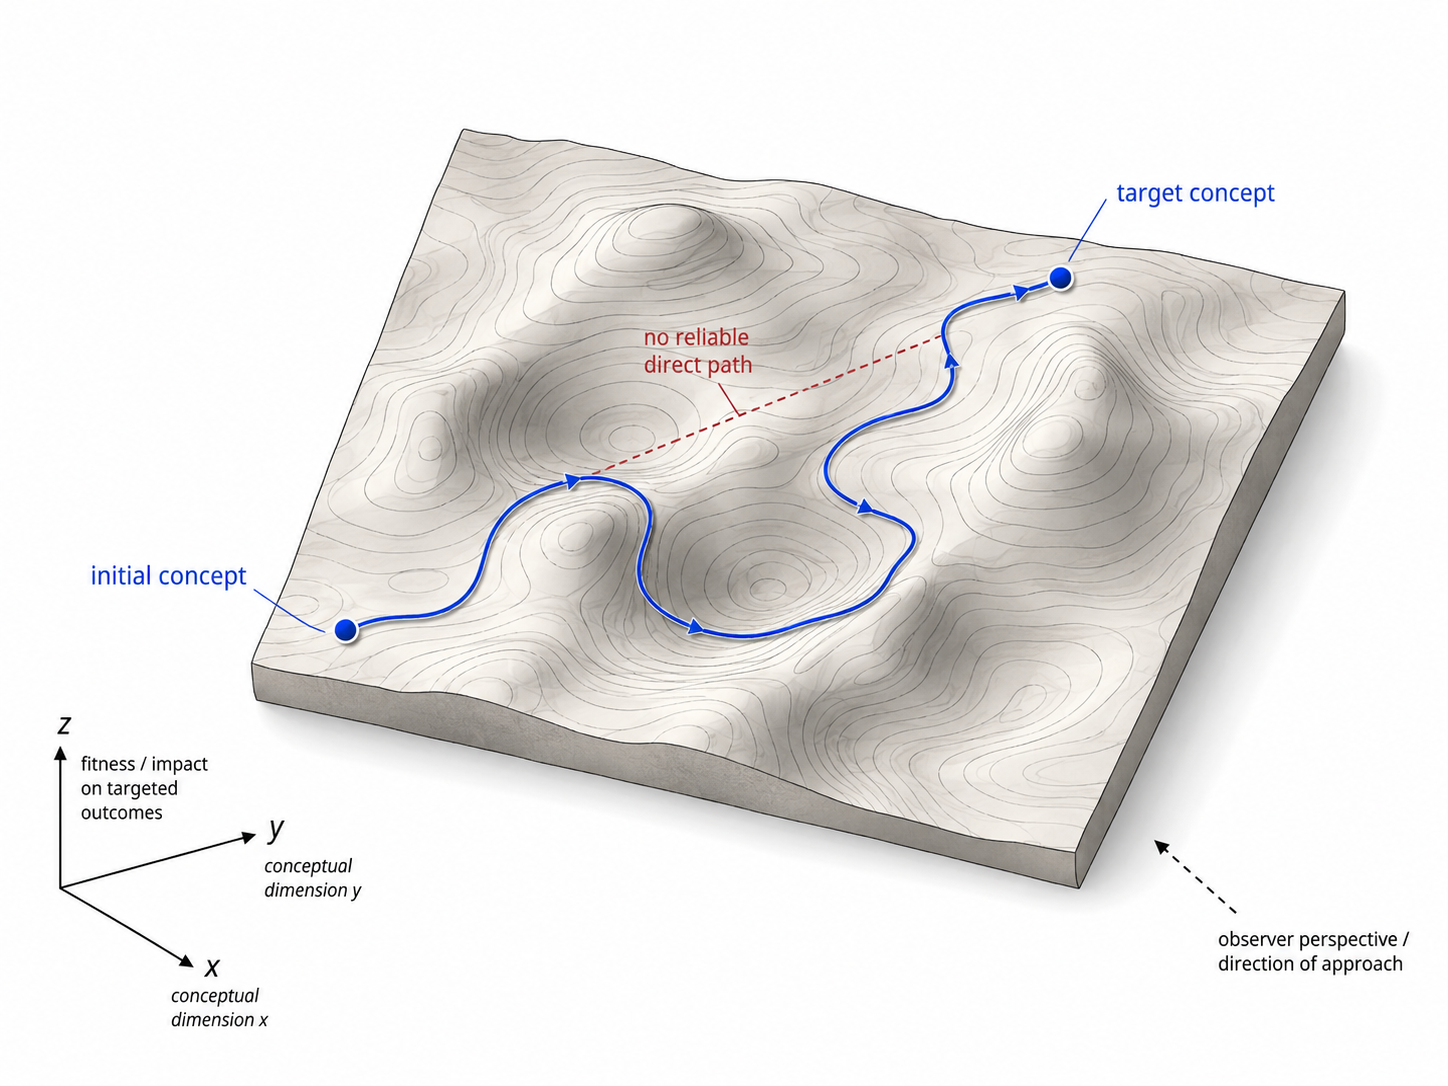
\includegraphics[width=0.92\textwidth]{risk_v87_topology_projection.png}
\caption{Fitness-conceptual topology projection. The horizontal axes represent a two-dimensional slice of conceptual space relative to the observer's direction of approach; the vertical axis represents fitness or impact on targeted outcomes. A problem exists when no reliable path is yet known between an initial concept and a target concept. The blue path shows a viable composed route through the shape; the dashed red line marks a direct route that is not yet reliable. The figure is explanatory rather than evidential.}
\label{fig:topology-projection}
\end{figure}

\subsection{From topology projection to a constraint algebra}
\label{sec:constraint-algebra}

A fitness-conceptual topology projection can be represented in two complementary ways. The first is the projected landscape: height represents the fitness gradient of candidate paths in terms of impact on targeted outcomes. The second is a typed graph laid over that landscape. Let
\begin{equation}
\mathcal{G}_{R}=(V,E,\tau,\beta),
\label{eq:risk-constraint-graph}
\end{equation}
where $V$ is a set of represented risk objects or boundary states, $E$ is a set of directed admissible transitions, $\tau:E\rightarrow\mathcal{T}$ assigns each transition an operator or method type, and $\beta$ assigns the boundary conditions under which that transition is valid.

Each node is therefore not merely a point on the map. It is a declared boundary: a state of the risk object, evidence record, intervention, or assessment process at which particular operations become admissible, inadmissible, unresolved, or escalation-requiring. Each edge is not merely a connection. It is a boundary condition on movement from one node to another: a statement that a particular method, model, measurement, or institutional procedure may be used to move from one represented state to the next only under its declared bridge, regime, provenance, and empirical-anchor conditions.

\begin{figure}[htbp]
\centering
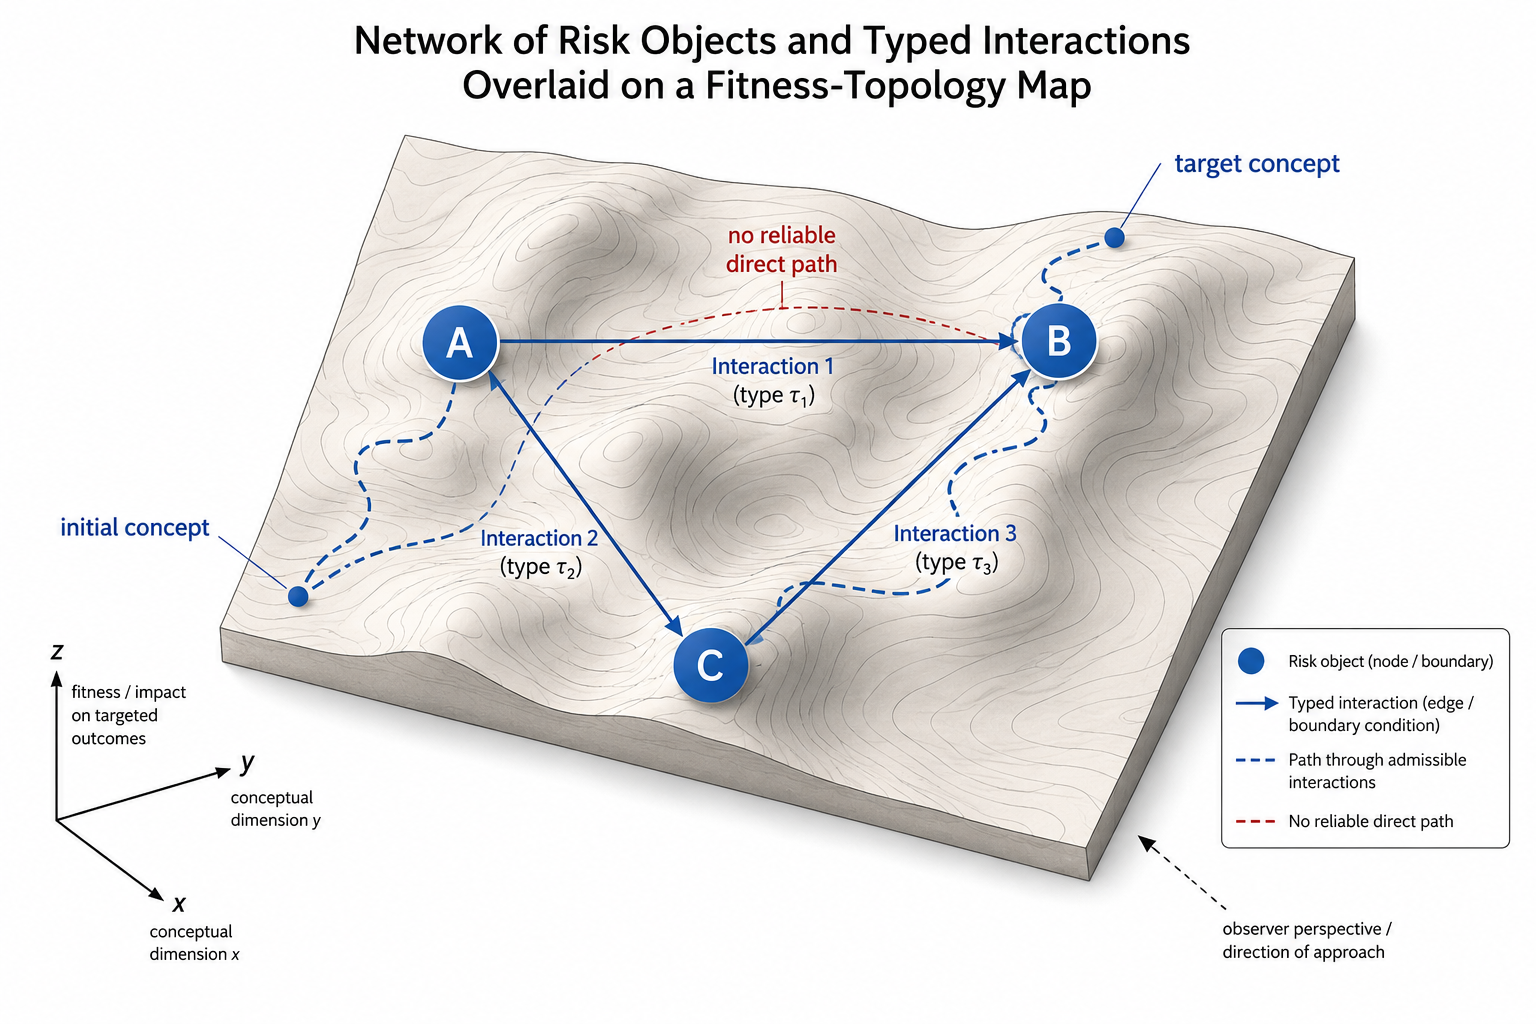
\includegraphics[width=0.96\textwidth]{risk_v87_constraint_graph.png}
\caption{Typed risk-object graph overlaid on a fitness-conceptual topology projection. Nodes represent declared boundaries or risk-object states; directed edges represent typed admissible interactions or boundary conditions. A composed route can be assessed piecewise through the methods valid in its respective regions, even where no reliable direct path is available. The graph is a constraint representation, not evidence that every node, edge, or path has been empirically anchored.}
\label{fig:risk-topology-constraint-graph}
\end{figure}

The graph generates a \emph{constraint algebra}: the set of typed compositions that remain admissible under the declared boundary conditions. Thus, a transition from risk object $A$ to risk object $Z$ need not require a single unified model of the entire conceptual space. It may instead be represented as a composition
\begin{equation}
A \xrightarrow[\beta_1]{\tau_1} B
\xrightarrow[\beta_2]{\tau_2} C
\xrightarrow[\beta_3]{\tau_3} \cdots
\xrightarrow[\beta_m]{\tau_m} Z,
\label{eq:piecewise-risk-composition}
\end{equation}
where each $\tau_i$ is a current risk-management method or interaction that is valid only in its declared region and under its declared conditions. This does not imply that every composed path is safe, complete, or empirically established. A missing edge, invalid bridge, regime change, failed empirical anchor, or prohibited composition remains a visible constraint rather than being silently smoothed over. The value of the representation is conditional: it permits existing domain-specific methods to be composed piecewise without requiring a prior unifying theory of every risk domain, while preserving the boundaries at which ordinary empirical assessment, institutional review, or escalation is still required.

The recursive step is needed when a one-shot local move does not preserve enough of the shape to decide the relevant question. In that case, global coherence is not a claim that everything must be inspected at once. It is a bounded procedure for circling the shape, preserving the parent object, testing load-bearing boundaries, and updating the map until the next move is typed: refine the map, route a missing anchor, produce a defeating witness, or stop.

\begin{figure}[htbp]
\centering
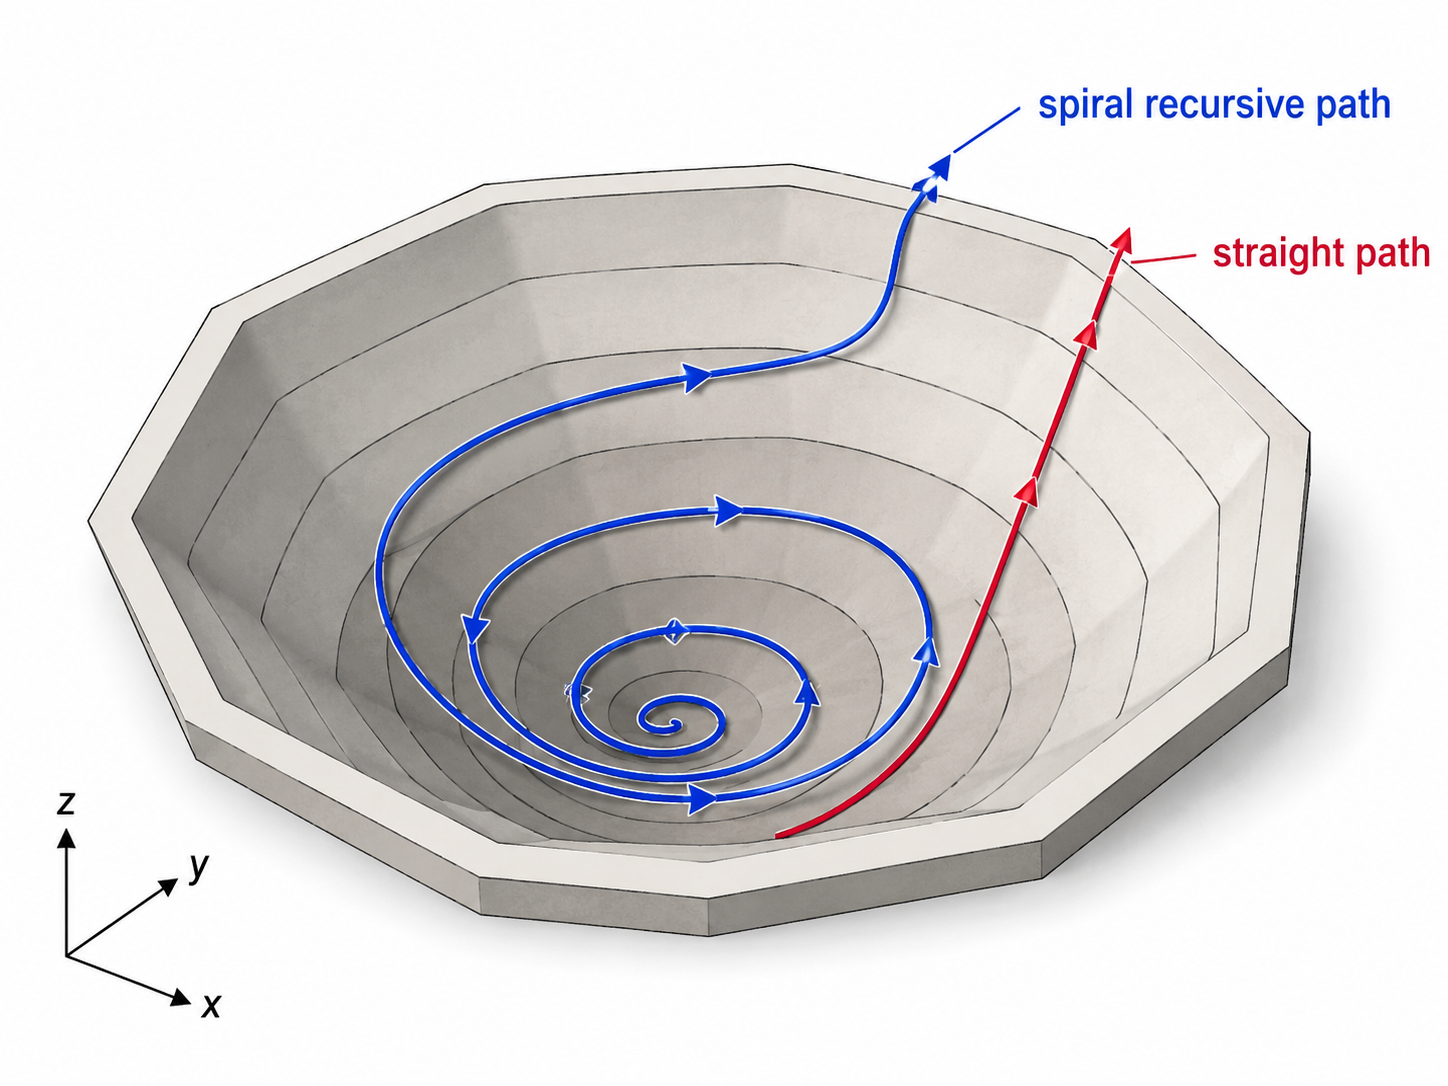
\includegraphics[width=0.92\textwidth]{risk_v87_bagua_pit.png}
\caption{Pit-shaped topology and recursive escape path. The straight path up the wall represents the tempting one-shot move that need not reliably exit the problem. The spiral path represents recursive traversal: repeated, typed passes that gradually preserve more of the topology until an exit route becomes available. This is a pedagogic visualization of non-factorizing assessment, not a literal terrain model, universal solver, or policy recommendation.}
\label{fig:pit-topology}
\end{figure}

The figures supply an intuitive visual for the recursive step. The ``pit'' is not circular reasoning and does not imply that every problem requires global coherence. It depicts the narrower case in which a direct local move has not preserved enough of the topology to decide the risk-relevant shape. A valid recursive pass must have a typed output: it adds a missing distinction or boundary, produces a completion-invariant constraint, requests an empirical anchor, routes the candidate to a different method, records a defeating witness, or terminates under a declared budget. Related semantic backpropagation work describes recursive semantic update as an implementable procedure rather than a purely literary metaphor \cite{williams2025semantic}; related work on wicked problems motivates the concern that local optimization can fail to recover a viable system-level path \cite{williams2023wicked}. Neither reference validates the present AI-risk examples or makes this protocol a substitute for empirical assessment.

\section{Second-order risk management and the risk object}

\label{sec:second-order}

\subsection{Definition}

\emph{Second-order risk management} is management of the processes that preserve, type, route, update, and escalate candidate risk objects. Its object is not only a hazard, exposure, consequence, or intervention. It is the assessment architecture through which such objects become available for first-order risk analysis.

\begin{table}[htbp]
\centering
\caption{First- and second-order risk management.}
\label{tab:first-second}
\begin{tabularx}{\textwidth}{>{\raggedright\arraybackslash}p{0.23\textwidth}p{0.32\textwidth}X}
\toprule
Level & Object managed & Core question \\
\midrule
First-order & Hazard, exposure, consequence, scenario, model, intervention, or governance choice & What is the risk, and what should be done within the specified decision frame? \\
Second-order & The formation, preservation, typing, routing, and update of the candidate object and its assessment frame & Can the relevant object remain available, bounded, and correctly typed long enough for first-order assessment to occur? \\
\bottomrule
\end{tabularx}
\end{table}

This does not imply that conventional risk methods are intrinsically local or inadequate. Rather, many methods receive a risk object, a scenario set, a model family, a decision context, or a quantity to estimate. Claim-status routing operates when that input is itself unstable or when the assessment gate risks collapsing distinctions among object, carrier, anchor, action, and route.

\subsection{Parent projection, carrier, and status substitution}

Let $P$ denote the \emph{parent projection}: the declared fitness-conceptual topology projection through which the candidate risk is represented. In the present paper, $P$ is not just a sentence or a chart; it is the risk-relevant shape together with the path question being asked of it. Let $K$ denote a bounded carrier, such as a figure, local chart, toy calculation, policy frame, wording choice, prototype model, or journal manuscript. The carrier may be defective without $P$ being defeated. Likewise, a decision-use objection may correctly block action without proving that $P$ is false or unworthy of assessment.

A \emph{projection-defeating witness} must be finite, stable in target, directed at $P$ or its load-bearing map, and contradiction-establishing at the claimed status. This is intentionally stricter than an objection token. It creates a finite stopping condition for residual carrier, venue, proof-status, or stylistic objections: they may remain actionable at their own coordinate, but do not become a terminal parent defeat without the required witness.

\section{Claim-status routing and the finite risk-status certificate}
\label{sec:certificate}

The risk-status certificate is the finite externalized object by which second-order risk management prevents loss of a sparse-prior candidate while blocking unjustified belief and action. It is not a probability estimate, a validation certificate, a publication recommendation, or a policy authorization.

Let a certificate be
\begin{equation}
C=(P,S,W,T),
\label{eq:certificate}
\end{equation}
where $P$ is the parent projection, $S$ is a status vector, $W$ is an optional defeat witness, and $T$ is an append-only routing trace. The status vector is
\begin{equation}
S=(s_P,s_R,s_E,s_D,s_A,s_G,s_Q),
\label{eq:status-vector}
\end{equation}
where $s_P$ is parent-projection status, $s_R$ representation status, $s_E$ empirical-anchor status, $s_D$ decision-use status, $s_A$ assessment-safety status, $s_G$ propagation status, and $s_Q$ the assigned review route. The  assessment-safety coordinate records whether a safe evidence route is declared, whether the proposed evidence plan is assessment-hazard coupled, or whether the relation is undetermined; it is not a hazard estimate or experimental approval.

\begin{figure}[htbp]
\centering
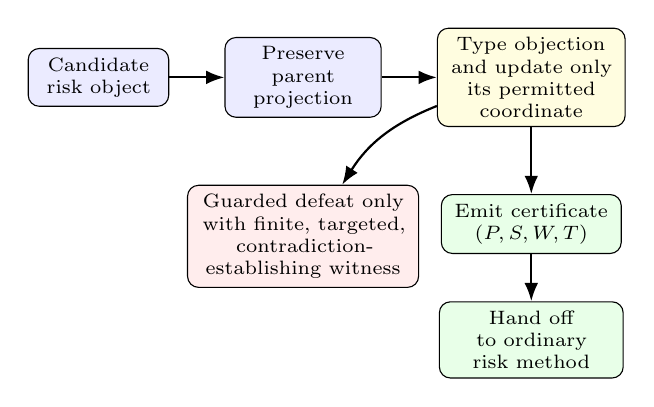
\begin{tikzpicture}[node distance=0.38cm and 0.7cm,every node/.style={font=\scriptsize},box/.style={draw,rounded corners,align=center,minimum height=0.7cm},arr/.style={-Latex,thick}]
\node[box,fill=blue!8,text width=1.55cm] (cand) {Candidate risk object};
\node[box,fill=blue!8,text width=1.75cm,right=of cand] (parent) {Preserve parent projection};
\node[box,fill=yellow!12,text width=2.15cm,right=of parent] (route) {Type objection and update only its permitted coordinate};
\node[box,fill=green!9,text width=2.05cm,below=0.85cm of route] (cert) {Emit certificate $(P,S,W,T)$};
\node[box,fill=green!9,text width=2.1cm,below=0.6cm of cert] (handoff) {Hand off to ordinary risk method};
\node[box,fill=red!7,text width=2.7cm,below=0.85cm of parent] (defeat) {Guarded defeat only with finite, targeted, contradiction-establishing witness};
\draw[arr] (cand)--(parent);
\draw[arr] (parent)--(route);
\draw[arr] (route)--(cert);
\draw[arr] (cert)--(handoff);
\draw[arr] (route) to[bend right=18] (defeat);
\end{tikzpicture}
\caption{Coordinate-wise certificate routing. Ordinary routing preserves parent identity and does not itself create projection defeat or external decision authorization.}
\label{fig:certificate-routing}
\end{figure}

A certificate answers the following questions.
\begin{enumerate}[label=(\arabic*)]
\item What is the parent projection, and what is explicitly outside it?
\item Which bounded carrier transmits the projection, and what may that carrier not prove?
\item Which empirical anchors are declared, immature, absent, disputed, or adequate for a specified downstream assessment?
\item Which coordinate has an objection actually targeted?
\item Which uses are authorized, blocked, or reserved for a domain process?
\item What partial fitness-conceptual topology, typed operators, and boundary conditions have been declared; which map-level constraints are completion-invariant; and which remain unresolved across admissible completions?
\item Does the proposed evidence route preserve the declared path and shape distinctions, and is it safe enough to be used as an assessment route rather than merely proposed as a traversal?
\item What finite witness would repair, localize, downgrade, stop, or defeat the object?
\item Which route receives the candidate next, which safety-case material must regenerate across successors, and which unresolved coordinates must accompany that handoff?
\end{enumerate}

\subsection{Ordinary routing and guarded defeat}

The ordinary router is a total operation
\begin{equation}
A:X_R\times O\longrightarrow X_R,
\end{equation}
where $X_R$ is the certificate-state space and $O$ is the set of typed objections. Ordinary routing may repair a carrier, request an empirical anchor, block decision use, localize a local chart, transfer venue, or route a non-decomposability concern for review. It does not itself set $s_P=\mathrm{defeated}$.

A separate guarded transition
\begin{equation}
D:X_R\times V\longrightarrow X_R
\end{equation}
may set $s_P=\mathrm{defeated}$ only when $V$ contains a witness satisfying the declared conditions
\begin{equation}
\operatorname{valid}(w)=\operatorname{stableTarget}(w)\wedge\operatorname{finite}(w)\wedge\operatorname{targetsParent}(w)\wedge\operatorname{contradiction}(w).
\label{eq:defeat-witness}
\end{equation}
Equation~\eqref{eq:defeat-witness} is a model-level gate, not an empirical truth detector. It specifies what the certificate must record before a parent-defeat state is entered.

\section{Functional-state-space capacity, predictive shape libraries, and bounded automation}
\label{sec:fss-capacity}

The supplement gives a bounded functional-state-space reconstruction of second-order risk management. In the main text, the practical point is narrower: only a limited family of operations can be partially externalized and reused without pretending to automate risk truth itself. Those operations act on certificate states, admissible transitions, typed updates, protected invariants, and explicit boundaries against unauthorized inferences.

The protected invariant set contains, at minimum:
\begin{align}
&\text{parent identity preservation},\\
&\text{coordinate-locality restrictions},\\
&\text{guarded projection defeat},\\
&\text{decision-use blocking under discovery or immature anchors},\\
&\text{no conversion of an assessment-hazard-coupled evidence plan into approval by ordinary routing},\\
&\text{well-formedness of defeated certificates}.
\end{align}

The reusable unit is not a superficial analogy or a generic visual pattern. It is a \emph{typed risk-shape record}: a bounded fragment of a fitness-conceptual topology projection together with the operators, boundaries, bridge and regime conditions, expected empirical signatures, empirical-anchor obligations, permitted uses, prohibited inferences, and stopping conditions on which its constraint depends. A library accumulates such records so that a new candidate need not force complete reconstruction of every already-understood topological relation.

\begin{figure}[htbp]
\centering
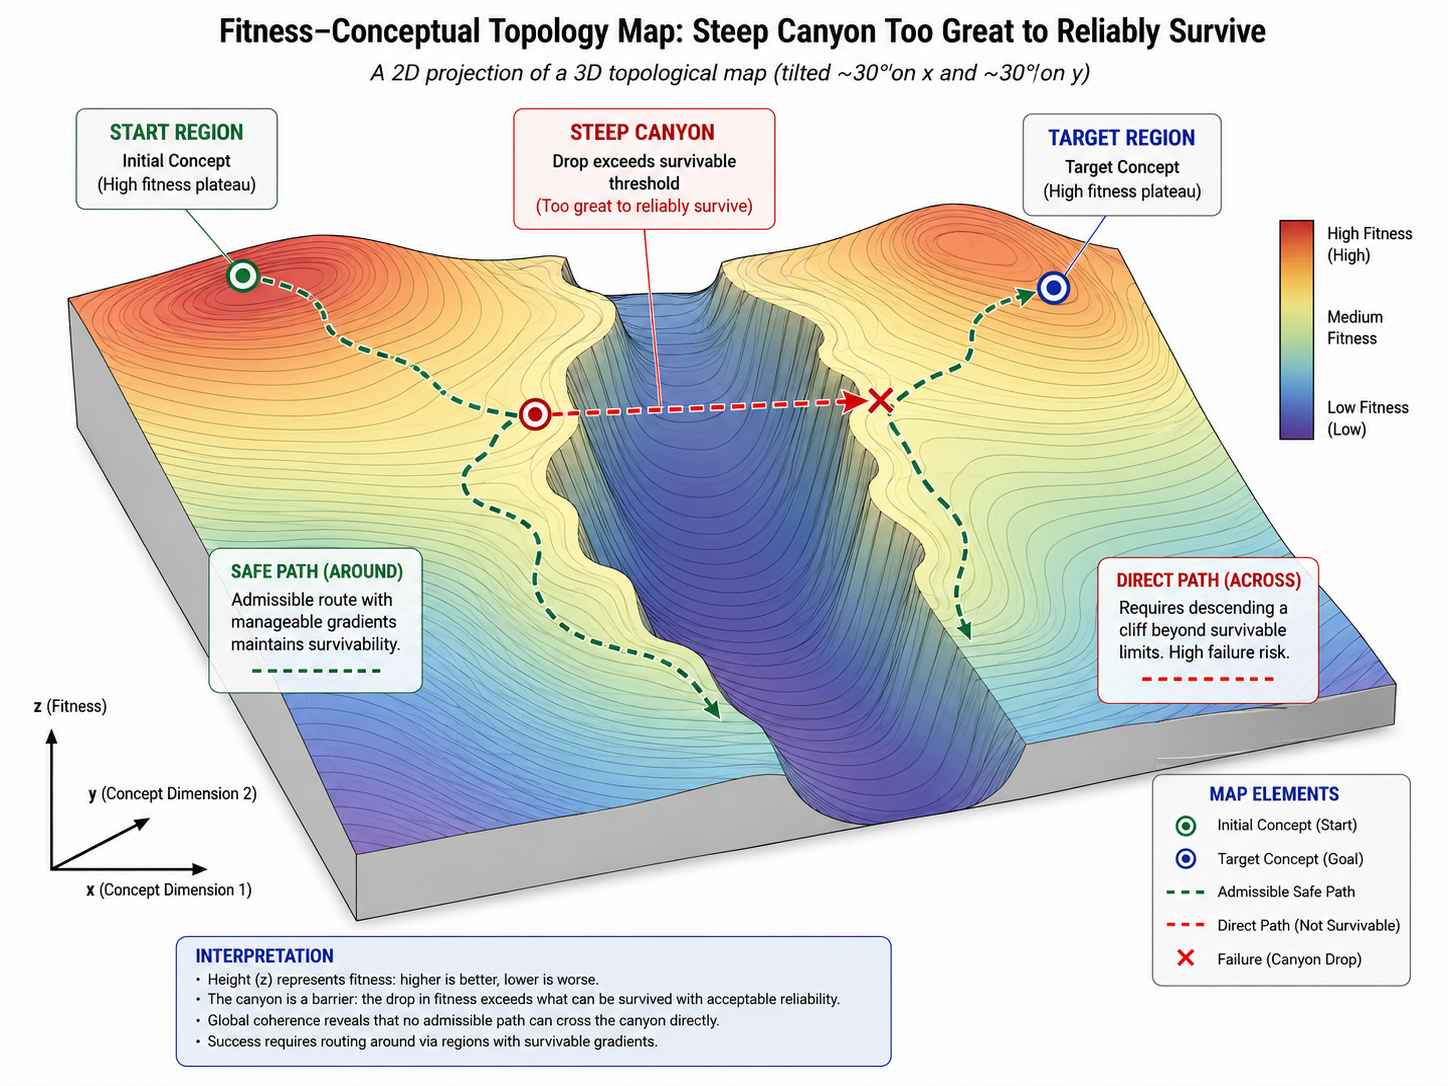
\includegraphics[width=0.96\textwidth]{risk_v87_canyon.png}
\caption{\textbf{Illustrative predictive risk shape: an inadmissible canyon crossing.} The topology represents a case in which the direct conceptual route crosses a fitness drop beyond the declared survivability boundary, while an indirect route remains within manageable gradients. Such a shape may be entered into a typed risk-shape library before empirical traversal or failure, provided its predicted status, bridge conditions, expected signatures, empirical-anchor obligations, and prohibited decision uses remain explicit. The figure does not establish that any real-world canyon, risk, or intervention has been empirically anchored.}
\label{fig:predictive-canyon}
\end{figure}

Crucially, a risk shape need not first be empirically measured before it can be entered into the library. A \emph{predicted shape} is prospectively identified from a declared partial map and its constraint algebra, with the empirical signatures that would register, narrow, or defeat the prediction made explicit. A \emph{registered shape} has relevant signatures observed, although its bridge or regime may still be unresolved. An \emph{anchored shape} has the bridge, regime, and empirical-anchor support required for its declared downstream use. These are status states, not truth values. To avoid an ambiguity, \emph{structural detection} here means prospective identification of a predicted shape from the declared map; \emph{empirical registration} means observation of the expected signatures. A predicted entry can support monitoring, safe evidence-route design, targeted measurement, adversarial review, and structural comparison; it cannot by itself support an empirical risk claim, a calibrated probability, a severity determination, or intervention authorization.

Reuse is therefore conditional on a compatibility mapping that preserves the roles on which the stored constraint depends. Successful reuse transfers only the applicable constraint, question, expected-signature ledger, or routing operation. It does not transfer empirical truth, probability, severity, or permission to act. A composition that introduces a new global coupling, changes the bridge or regime, or exceeds the declared compatibility conditions must be escalated rather than treated as a routine library match.

\begin{figure}[htbp]
\centering
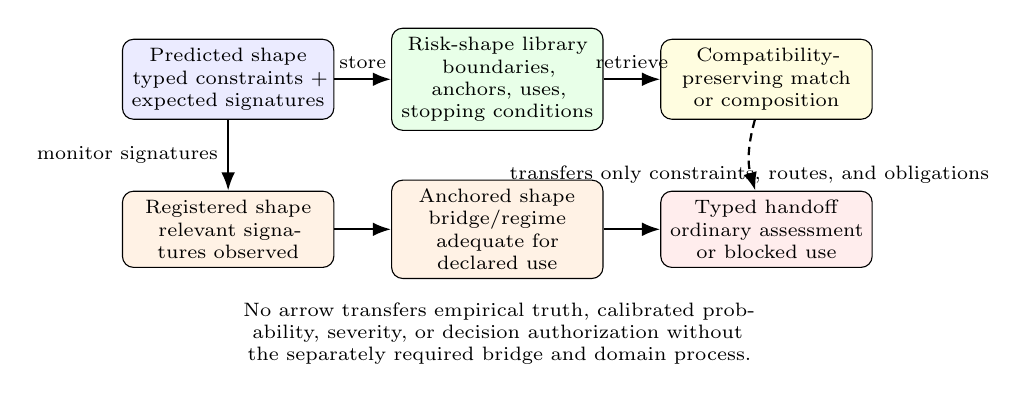
\begin{tikzpicture}[
  node distance=0.56cm and 0.72cm,
  every node/.style={font=\scriptsize},
  box/.style={draw,rounded corners,align=center,minimum height=0.86cm,text width=2.45cm},
  arr/.style={-Latex,thick}
]
\node[box,fill=blue!8] (pred) {Predicted shape\\typed constraints + expected signatures};
\node[box,fill=green!9,right=of pred] (library) {Risk-shape library\\boundaries, anchors, uses, stopping conditions};
\node[box,fill=yellow!12,right=of library] (match) {Compatibility-preserving match or composition};
\node[box,fill=orange!10,below=0.9cm of pred] (reg) {Registered shape\\relevant signatures observed};
\node[box,fill=orange!10,right=of reg] (anch) {Anchored shape\\bridge/regime adequate for declared use};
\node[box,fill=red!7,right=of anch] (route) {Typed handoff\\ordinary assessment or blocked use};
\draw[arr] (pred)--node[above,font=\scriptsize]{store} (library);
\draw[arr] (library)--node[above,font=\scriptsize]{retrieve} (match);
\draw[arr] (pred)--node[left,font=\scriptsize]{monitor signatures} (reg);
\draw[arr] (reg)--(anch);
\draw[arr] (anch)--(route);
\draw[arr,densely dashed] (match) to[bend right=16] node[below,font=\scriptsize,align=center]{transfers only constraints, routes, and obligations} (route);
\node[align=center,font=\scriptsize,text width=7.7cm,below=0.18cm of anch] {No arrow transfers empirical truth, calibrated probability, severity, or decision authorization without the separately required bridge and domain process.};
\end{tikzpicture}
\caption{Predictive risk-shape library workflow. A shape may be prospectively identified before empirical registration, but its certificate must retain expected signatures, empirical-anchor obligations, and blocked uses. Reuse or composition is allowed only under a compatibility mapping that preserves the constraints being transferred.}
\label{fig:predictive-library}
\end{figure}

The relevant scalability claim is therefore not that automation can determine risk truth. It is that finite, typed, auditable operations can be externalized and reused: preserving, comparing, retrieving, compatibility-checking, composing, routing, clustering, update, contradiction detection, trace maintenance, and escalation. The unit of work changes from reconstructing each candidate case from scratch to retrieving and validating bounded records while reserving scarce human or independent assessment for contested coordinates.

Let $N$ be the number of candidate objects, $h$ the average cost of full expert reconstruction, $M\ll N$ the number of candidates that remain contested after routing, and let the remaining terms denote the cost of building, retrieving, matching, validating, and composing library records. Then the conditional contrast is
\begin{align}
C_{\mathrm{reconstruct}}(N)&\approx \sum_{j=1}^{N}C_{\mathrm{new}}(S_j),\\
C_{\mathrm{library}}(N)&\approx C_{\mathrm{build}}(\mathcal{L})+\sum_{j=1}^{N}\bigl(C_{\mathrm{retrieve},j}+C_{\mathrm{match},j}+C_{\mathrm{validate},j}+C_{\mathrm{compose},j}\bigr)+Mh.
\label{eq:capacity}
\end{align}

Equation~\eqref{eq:capacity} is not an empirical efficiency finding. It is a conditional capacity model. Its premise is finite encodability, stable parent identity, invariant-preserving compatibility checks, typed routing, auditable update rules, bounded propagation hazard, maintained expected-signature and anchor ledgers, and a genuine reduction in the cases requiring full reconstruction. The number of potentially compatible compositions can grow faster than the number of stored shapes. Under the stated conditions, this is a potential source of significant capacity expansion in novel domains; it remains only a coverage potential, because no composition is reusable until its additional couplings and status boundaries are checked. The advantage disappears or pauses when a risk shape is non-factorizing, unbounded, unstable under reformulation, dependent on an unrepresented global interaction, or used beyond the empirical status and permitted scope recorded in its certificate.

A representation that increases throughput while permitting unauthorized cross-coordinate collapse is not a capacity gain. It is an expansion of the risk-management attack surface.

\section{Partial conceptual topology, shape-sensitive adequacy, safe evidence, and regenerative propagation}
\label{sec:composition}

The partial conceptual topology of \cref{sec:partial-topology} is a representation of constraints, not an assertion that the full AI-risk space has been simulated. It explains how a certificate may preserve a map-level claim before every possible capability, deployment, and governance state is implemented: the certificate must state the relevant slice of the map, the admissible ways it may be completed, and the constraints whose satisfaction is preserved across that declared class. This permits prospective structural identification of a predicted shape before its empirical signatures are registered, but it does not remove the unresolved bridge or anchor obligations recorded in the certificate. Any conclusion that depends on a missing operator family, an omitted bridge to deployment reality, or an unconstrained empirical coordinate remains routed rather than emitted as a settled result.

Some risk questions are questions about the \emph{shape} of a route rather than about any single local point on the map. Examples include whether an intervention remains effective across its route, whether a capability path remains controllable as it moves through multiple regimes, or whether a governance path retains enough coverage as conditions change. The supplement formalizes these as shape-level questions over a declared composition signature. The main-text point is simpler: a local summary is inadequate when it flattens distinctions in the shape that change the answer to the declared question. In practice, those distinctions often concern bridge validity, validity regime, ordered history and retention, and required support or coverage.

A second boundary concerns evidence acquisition. Some proposed evidence routes are themselves hazard-coupled: the act of traversing the unresolved branch may amplify or irreversibly worsen the very condition being assessed. When that boundary is active, ordinary routing must not convert the proposed experiment, deployment, or capability demonstration into an approved evidence route. The appropriate output is a \emph{safe decision object} request: for example, a bounded surrogate, simulation, barrier or containment argument, distributed measurement plan, or another declared route that decides the relevant shape-level question without traversing the unresolved hazardous branch. The absence of a supplied safe witness does \emph{not} establish that no safe route exists; it blocks presumption of safety while the route remains unresolved.

A third boundary is temporal. Retaining an artifact, procedure, model, or institutional record is not equivalent to retaining the complete constraint certificate through which a successor can reconstruct the parent shape, inspect its bridge and regime conditions, criticize or correct it, and transmit the corrected object. We call this stronger condition \emph{regenerative safety-case propagation}. A propagation record must therefore distinguish trace retention, operational retention, and regenerative propagation. This matters for AI-risk management when safety, monitoring, or intervention conditions must survive across model versions, operators, institutions, or jurisdictions. It does not claim that a particular safety case has failed to propagate; it makes the missing bridge visible and routes it for assessment.

\section{Conservative refinement and the companion Lean artifact}

\label{sec:lean}

The accompanying Lean 4 artifact formalizes a small, non-load-bearing kernel of the certificate protocol. It introduces separate projection, representation, empirical-anchor, decision-use, propagation, and review-route coordinates; a guarded defeat witness; an append-only trace; and a conservative projection to a simpler single-route view. The manuscript's partial-topology, predictive-library, shape-sensitive adequacy, assessment-safety, and regenerative-propagation distinctions are conditional architecture unless and until they are separately declared and verified in a conservative formal extension. In particular, the current artifact does not enumerate admissible completions of a partial conceptual topology or certify completion-invariance; the manuscript identifies those as explicit future formalization targets. The artifact establishes consequences of its declared definitions, including:
\begin{enumerate}[label=(\alph*)]
\item ordinary routing preserves parent identity;
\item representation-only objections preserve projection and empirical-anchor status;
\item ordinary routing does not create external decision authorization;
\item discovery propagation blocks decision use;
\item guarded defeat is well formed only with a typed valid witness;
\item shared non-defeat routes conservatively refine the earlier routing categories; and
\item deliberately unsafe carrier-to-defeat and discovery-to-authorization mutations violate the intended invariants.
\end{enumerate}

The artifact is a bounded corroboration layer. It does \emph{not} establish that a real-world objection has been correctly typed, that a witness is empirically adequate, that independent checking has occurred, that a fixed point has been reached, that Equation~\eqref{eq:capacity} holds in practice, or that any AI, Great Filter, governance, or public-health risk claim is true. The supplement maps each formal statement to its manuscript role and non-entailments.

A future extension is admissible only as a conservative refinement: it must declare the new state or transition; the coordinates it may alter; the coordinates it must preserve; an attack or mutation witness produced by violation; and its projection back to the baseline kernel. This is how the formal component bounds, rather than merely accumulates, new attack surfaces.

\section{Threat-coupled admission contraction and governance coverage}
\label{sec:threat-coverage}

High-valence risks can alter the assessment gate before the parent projection is tested. Let the gate state be
\begin{equation}
a_t=(p_t,\rho_t,\Lambda_t,M_t),
\end{equation}
where $p_t$ is perceived personal, institutional, reputational, or paradigmatic threat; $\rho_t$ is method-risk aversion; $\Lambda_t$ is an admissible method-risk threshold; and $M_t$ is the permitted method set. The threat-coupled admission-contraction hypothesis is
\begin{equation}
\frac{\partial \rho_t}{\partial p_t}>0,\qquad \frac{\partial |M_t|}{\partial \rho_t}<0.
\label{eq:contraction}
\end{equation}
A blind spot occurs when a method required to preserve or assess a candidate is excluded before its parent projection is tested.

This is a conditional mechanism hypothesis, not an inference from reader response to the truth of any high-valence object-level risk. Its importance is procedural: threat may alter the method set that decides what can enter assessment. AI-pause and Great Filter cases are diagnostic stressors because they activate precisely this possibility. Their role is to test whether carrier, valence, proof-status, or decision-use objections are correctly routed rather than converted into parent defeat.

Let governance coverage under architecture $\pi$ be
\begin{equation}
I_\pi(t)=\frac{C_G^\pi(t)}{C_R(t)},
\label{eq:coverage}
\end{equation}
where $C_G^\pi(t)$ is represented correction and governance coverage, and $C_R(t)$ is the coverage required by the evolving risk topology. A loss-sensitive uncovered-risk quantity is
\begin{equation}
L_{\mathrm{uncovered}}(t)=\int_{\Risk\setminus\Risk_{\mathrm{covered}}(t)}w(r)\,d\mu_t(r).
\label{eq:uncovered}
\end{equation}
The claim is conditional: when required topology grows faster than preserved, typed, and updateable assessment coverage, apparent risk-management activity can coexist with declining effective coverage. This paper does not establish that such a collapse is currently occurring. It provides a representation and routing architecture for making the condition assessable. Under the illustrative exponential parameterization $C_R(t)=C_R(0)e^{g_Rt}$ and $C_G^\pi(t)=C_G^\pi(0)e^{g_G^\pi t}$, normalized at $t=0$, the coverage condition is
\begin{equation}
\Gamma_\pi(t)=I_\pi(t)=e^{(g_G^\pi-g_R)t}.
\label{eq:gamma-coverage}
\end{equation}
The sign condition $g_G^\pi-g_R$ is a target for measurement and review; Equation~\eqref{eq:gamma-coverage} is not a forecast.

\section{Worked cases: anchor and portability}
\label{sec:cases}

\subsection{Anchor case: intervention durability and AI-pause}

The generic parent question is not ``does a particular pause work?'' It is whether an intervention's initial coverage persists when the problem topology expands, fragments, adapts, or routes around the intervention. A local chart can represent an intervention-durability kernel,
\begin{equation}
S(t)=Ae^{-kt},
\label{eq:pause-suppression}
\end{equation}
where $A\in[0,1]$ is the initial fraction of counterfactual frontier-relevant activity removed and $k>0$ is aggregate erosion under a declared boundary. For cumulative residual activity, the unweighted compression is
\begin{equation}
R(T)=1-A\frac{1-e^{-kT}}{kT},\qquad R(0)=1-A,
\label{eq:pause-residual}
\end{equation}
and, for residual threshold $\eta$,
\begin{equation}
P_{\mathrm{eff}}(T;\eta)=\Pr[R(T)\leq\eta].
\label{eq:pause-effectiveness}
\end{equation}
The kernel is a bounded carrier: $A$, $k$, the erosion form, and any weighting by counterfactual activity or risk intensity remain empirical-anchor and mapping questions. Its value is to distinguish a one-time compliance rate from a threshold-crossing durability relation.

\begin{figure}[htbp]
\centering
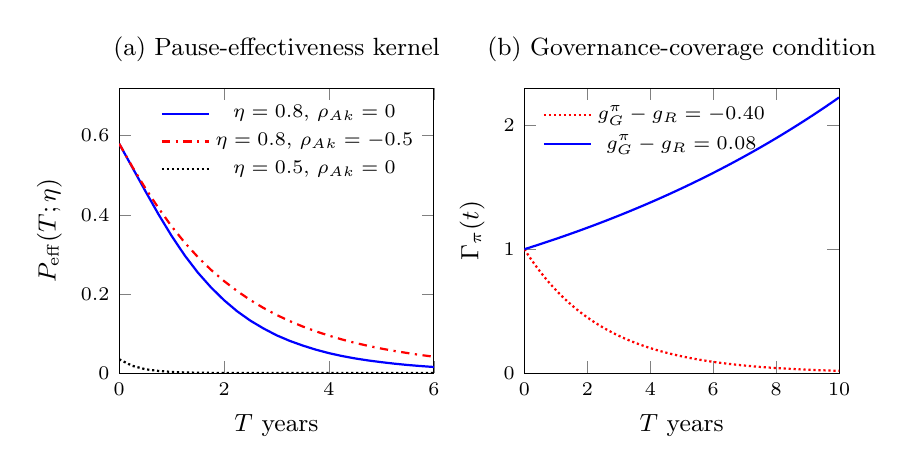
\begin{tikzpicture}
\begin{groupplot}[
  group style={group size=2 by 1, horizontal sep=1.15cm},
  width=0.46\textwidth,height=5.2cm,
  tick label style={font=\scriptsize},label style={font=\small},
  legend style={font=\scriptsize,draw=none,fill=none},
  every axis plot/.append style={thick}
]
\nextgroupplot[
  xmin=0,xmax=6,ymin=0,ymax=0.72,
  xlabel={$T$ years},ylabel={$P_{\mathrm{eff}}(T;\eta)$},
  title={(a) Pause-effectiveness kernel},
  title style={font=\small},
  legend style={at={(0.98,0.98)},anchor=north east}
]
\addplot[blue] coordinates {(0.00,0.5796) (0.25,0.5198) (0.50,0.4596) (0.75,0.4011) (1.00,0.3465) (1.25,0.2972) (1.50,0.2539) (1.75,0.2166) (2.00,0.1841) (2.25,0.1561) (2.50,0.1326) (2.75,0.1129) (3.00,0.0956) (3.25,0.0815) (3.50,0.0696) (3.75,0.0592) (4.00,0.0504) (4.25,0.0431) (4.50,0.0370) (4.75,0.0319) (5.00,0.0276) (5.25,0.0238) (5.50,0.0205) (5.75,0.0178) (6.00,0.0154)};
\addlegendentry{$\eta=0.8$, $\rho_{Ak}=0$}
\addplot[red,dashdotted] coordinates {(0.00,0.5796) (0.25,0.5213) (0.50,0.4669) (0.75,0.4168) (1.00,0.3707) (1.25,0.3297) (1.50,0.2932) (1.75,0.2609) (2.00,0.2325) (2.25,0.2072) (2.50,0.1846) (2.75,0.1647) (3.00,0.1470) (3.25,0.1315) (3.50,0.1177) (3.75,0.1055) (4.00,0.0947) (4.25,0.0849) (4.50,0.0763) (4.75,0.0687) (5.00,0.0619) (5.25,0.0559) (5.50,0.0506) (5.75,0.0457) (6.00,0.0414)};
\addlegendentry{$\eta=0.8$, $\rho_{Ak}=-0.5$}
\addplot[black,densely dotted] coordinates {(0.00,0.0348) (0.25,0.0184) (0.50,0.0097) (0.75,0.0054) (1.00,0.0030) (1.25,0.0016) (1.50,0.0010) (1.75,0.0006) (2.00,0.0004) (2.25,0.0003) (2.50,0.0002) (2.75,0.0001) (3.00,0.0001) (3.25,0.0000) (3.50,0.0000) (3.75,0.0000) (4.00,0.0000) (4.25,0.0000) (4.50,0.0000) (4.75,0.0000) (5.00,0.0000) (5.25,0.0000) (5.50,0.0000) (5.75,0.0000) (6.00,0.0000)};
\addlegendentry{$\eta=0.5$, $\rho_{Ak}=0$}
\nextgroupplot[
  xmin=0,xmax=10,ymin=0,ymax=2.3,
  xlabel={$T$ years},ylabel={$\Gamma_\pi(t)$},
  title={(b) Governance-coverage condition},
  title style={font=\small},
  legend style={at={(0.03,0.98)},anchor=north west}
]
\addplot[red,densely dotted,domain=0:10,samples=100] {exp(-0.40*x)};
\addlegendentry{$g_G^\pi-g_R=-0.40$}
\addplot[blue,domain=0:10,samples=100] {exp(0.08*x)};
\addlegendentry{$g_G^\pi-g_R=0.08$}
\end{groupplot}
\end{tikzpicture}
\caption{Restored pause-effectiveness and governance-coverage kernels. Panel (a) is an illustrative calculation with $A\sim\mathrm{Beta}(2.6,8.15)$ and log-normal $k$ (median $0.651\,\mathrm{yr}^{-1}$, log-scale $\sigma=0.5$), coupled through a Gaussian copula. The curves compare independent and negatively correlated $(A,k)$ cases; they are not fitted forecasts. Panel (b) instantiates Equation~\eqref{eq:gamma-coverage} for two illustrative coverage gaps.}
\label{fig:pause-governance-kernels}
\end{figure}

Failure of a particular curve, parameterization, or visual representation repairs or defeats the chart unless it supplies a finite witness against the generic topology-expansion question itself. The certificate in this case blocks a number of inferences: it does not authorize a pause, estimate enforcement leakage, forecast technical capability, rank policies, or claim that a pause is sufficient. It may authorize only preservation of the durability question, targeted model development, empirical anchoring, adversarial review, comparison of intervention architectures, and handoff to ordinary decision analysis if decision-relevant inputs become available. The case is meaningful because it preserves the action-boundary question under a high-valence stressor without mistaking that preservation for policy. It also raises four structural questions: whether the partial conceptual topology declares enough typed operators and boundaries to support a completion-invariant durability constraint, whether the declared bridge/regime/history/coverage structure is preserved, whether assessment itself is hazard coupled, and whether the safety case can regenerate across successors.

\subsection{Portability case: emerging public-health signal}
\label{sec:public-health}

Consider a candidate public-health signal comprising persistent wastewater anomaly, genomic novelty, weak clinical indication, geographic dispersion, and reporting lag. The parent projection is not ``a severe pathogen exists.'' It is that the observed configuration may define a risk-relevant shape that merits preservation and formal assessment before hospital-severity estimates mature.

The case can be represented as a typed graph over a partial fitness-conceptual topology. Let node $A$ represent a persistent but initially weak surveillance anomaly; let node $C$ represent a provenance-controlled and sequence-reviewed signal with preliminary geographic or syndromic corroboration; and let node $B$ represent admission to formal public-health risk assessment. The relevant question is not whether a direct transition from $A$ to $B$ can be assumed. It is whether a composed route
\begin{equation}
A \xrightarrow[\beta_{\mathrm{lab}}]{\tau_{\mathrm{lab}}} C
\xrightarrow[\beta_{\mathrm{surv}}]{\tau_{\mathrm{surv}}} B
\label{eq:public-health-composition}
\end{equation}
is admissible, where $\tau_{\mathrm{lab}}$ includes contamination control, repeated detection, sequencing reproducibility, and provenance review, while $\tau_{\mathrm{surv}}$ includes dispersion assessment, syndromic or clinical corroboration, delay analysis, and surveillance escalation under the relevant public-health procedures.

The graph makes the limiting conditions explicit. A direct path from weak anomaly to severity conclusion is not reliable. Nor does the existence of a path from anomaly to formal assessment establish a pathogen, estimate severity, or authorize intervention. It establishes only that a declared piecewise route may be available for transforming a weak-signal object into a more structured assessment object, provided the boundary conditions on each edge are met.

\begin{table}[htbp]
\centering
\caption{Illustrative typed certificate for an emerging public-health signal.}
\label{tab:public-health}
\small
\begin{tabularx}{\textwidth}{>{\raggedright\arraybackslash}p{0.27\textwidth}X}
\toprule
Coordinate & Status \\
\midrule
Parent projection & The combined signal may define a risk-relevant shape that merits preservation and formal assessment before hospital-severity estimates mature. \\
Node $A$ & Persistent wastewater or other surveillance anomaly, initially bounded by contamination, sampling, and reporting uncertainty. \\
Edge $A\rightarrow C$ & Laboratory and provenance route: repeated detection, contamination controls, sequencing reproducibility, novelty assessment, and source discrimination. \\
Node $C$ & A more structured signal with defined provenance and preliminary cross-domain corroboration; it is not yet a severity conclusion. \\
Edge $C\rightarrow B$ & Surveillance and assessment route: geographic dispersion, syndromic or clinical corroboration, reporting-delay analysis, expert review, and admission to ordinary public-health assessment. \\
Node $B$ & Formal risk-assessment object for domain-specific surveillance, laboratory validation, epidemiological assessment, and public-health decision processes. \\
Blocked uses & Public alarm, emergency declaration, intervention authorization, calibrated severity claim, outbreak forecast, coercive action, or any assertion that a severe pathogen has been established. \\
Defeat / stopping conditions & No persistence anchor; novelty shown to be artefact or ordinary variation; dispersion collapses to a local source; a required edge condition fails; the parent shifts from assessment admission to severity assertion; or propagation hazard dominates discovery value. \\
\bottomrule
\end{tabularx}
\end{table}

This example shows how a partial risk topology can preserve a weak-signal candidate without requiring a complete epidemiological model or a single direct inference from anomaly to conclusion. The nodes identify the states at which assessment changes character; the edges identify the methods and boundary conditions required for movement between those states. The certificate preserves the parent projection, blocks unauthorized inference, and routes the object through the public-health methods appropriate to each region of the represented topology.

\section{Boundaries, failure modes, and evaluation program}
\label{sec:evaluation}

The method is not self-certifying. Its own defeat or downgrade conditions include inability to state a stable parent projection; inability to declare finite status consequences; a routing rule that converts a genuine projection defeat into an innocuous carrier condition; inability to distinguish discovery from decision authorization; unbounded reconstruction burden; empirically unavailable load-bearing anchors; or evidence that certificate-guided routing increases false propagation or reduces decision-relevant distinction.

A pilot evaluation can compare unstructured review with certificate-guided routing on synthetic and historical sparse-prior cases. Preregistered outcomes should include:
\begin{enumerate}[label=(\arabic*)]
\item parent-object preservation after independent restatement;
\item inter-rater agreement on objection target and status;
\item precision and recall of projection-defeat identification;
\item rate of status substitution;
\item time to stable classification;
\item expert reconstruction time per candidate;
\item false-admission and false-propagation rates;
\item representation-adequacy error: cases in which a reduced record identifies trajectories with different declared predicate values;
\item unsafe-evidence-route error: cases in which a hazard-coupled route is silently treated as an approved assessment method; and
\item regenerative safety-case retention: whether a successor can reconstruct, criticize, correct, and transmit the safety-relevant certificate rather than only recover an artifact or procedure; and
\item frequency with which the protocol correctly adds no material value.
\end{enumerate}

At least four negative controls are required: a mature well-specified risk for which the certificate adds little; an incoherent candidate that should be defeated; a carrier defect that should preserve the parent; and an unbounded or propagation-hazardous case that must be escalated rather than automatically routed.

\section{Conclusion}
\label{sec:conclusion}

Sparse-prior risk analysis can fail before conventional uncertainty analysis begins. The relevant failure is not simply an incorrect probability or poor policy choice; it is loss of the candidate object through status substitution. Human stakes determine why this loss matters. Global coherence identifies the structural difference between a local objection and parent defeat. Claim-status routing supplies a finite, coordinate-wise mechanism for preserving the distinction. Typed graph and library representations identify the bounded operations that can scale without claiming automatic risk truth. Ordinary risk-analysis methods then receive a better-preserved object on which to operate.

The protocol is intentionally narrow. Preserve the parent. Type the objection. Update only the permitted coordinate. Declare the partial conceptual topology, its admissible completion class, and the constraints that are invariant across that class. Block unsupported decision use. Require a finite, targeted witness for defeat. Escalate a reduction that collapses trajectories with different declared predicate values. Do not presume that a hazardous traversal is a safe evidence route. Distinguish retained artifacts from a safety case that successors can regenerate. These are not substitutes for empirical assessment or governance. They are conditions for ensuring that those processes can still encounter the object they are meant to assess.

\begin{thebibliography}{99}
\bibitem{bankes1993} Bankes, S. (1993). Exploratory modeling for policy analysis. \textit{Operations Research}, 41(3), 435--449.
\bibitem{benhaim2006} Ben-Haim, Y. (2006). \textit{Info-Gap Decision Theory: Decisions Under Severe Uncertainty}. Academic Press.
\bibitem{cooke1991} Cooke, R. M. (1991). \textit{Experts in Uncertainty: Opinion and Subjective Probability in Science}. Oxford University Press.
\bibitem{haasnoot2013} Haasnoot, M., Kwakkel, J. H., Walker, W. E., and ter Maat, J. (2013). Dynamic adaptive policy pathways. \textit{Global Environmental Change}, 23(2), 485--498.
\bibitem{hanson1998} Hanson, R. (1998). The Great Filter -- Are We Almost Past It? Manuscript, available from the author.
\bibitem{kaplan1981} Kaplan, S., and Garrick, B. J. (1981). On the quantitative definition of risk. \textit{Risk Analysis}, 1(1), 11--27.
\bibitem{lempert2003} Lempert, R. J., Popper, S. W., and Bankes, S. C. (2003). \textit{Shaping the Next One Hundred Years}. RAND.
\bibitem{marchau2019} Marchau, V. A. W. J., Walker, W. E., Bloemen, P. J. T. M., and Popper, S. W., eds. (2019). \textit{Decision Making under Deep Uncertainty}. Springer.
\bibitem{renn2008} Renn, O. (2008). \textit{Risk Governance: Coping with Uncertainty in a Complex World}. Earthscan.
\bibitem{saltelli2008} Saltelli, A., Ratto, M., Andres, T., Campolongo, F., Cariboni, J., Gatelli, D., Saisana, M., and Tarantola, S. (2008). \textit{Global Sensitivity Analysis: The Primer}. Wiley.
\bibitem{stirling2010} Stirling, A. (2010). Keep it complex. \textit{Nature}, 468, 1029--1031.
\bibitem{williams2025semantic} Williams, A. E. (2025). Semantic backpropagation: Extending symbolic network effects to achieve non-linear scaling in semantic systems. \textit{Computing and Artificial Intelligence}, 3(2), 2300--2300.
\bibitem{williams2023wicked} Williams, A. E. (2023). Are wicked problems a lack of general collective intelligence? GCI and wicked problems. \textit{AI \& Society}, 38(1), 343--348.
\end{thebibliography}

\end{document}
